%! TEX program = lualatex
\documentclass[12pt]{scrartcl}
% Packages
%\usepackage[margin=1.5in]{geometry}
\usepackage{index}
\usepackage{amsbsy} % Bold math symbols
\makeindex
%\usepackage[utf8]{inputenc}
\usepackage[T1]{fontenc}
\usepackage{tcolorbox}
\tcbuselibrary{theorems}
\tcbuselibrary{skins}
\tcbuselibrary{breakable}
\usepackage{varwidth}
\usepackage{textcomp}
\usepackage{amsmath, amssymb}
\usepackage{esint}
\usepackage{titlesec}
\usepackage{xcolor}
\usepackage{titling}
\usepackage[linktocpage]{hyperref}
\usepackage{pgfplots}
\usepackage{multicol}
\setlength{\columnsep}{2em}
\usepackage{caption}
\usepackage{amsthm}
\usepackage{import}
\usepackage{cancel}
\usepackage{caption}
\usepackage{nicematrix}
\usepackage{mathrsfs}
\usepackage{mathtools}
%\usepackage{parskip}
\usepackage{enumerate}
\usepackage{graphicx}
\usepackage[italian]{babel}
\usepackage{setspace}
\setstretch{1.2}
% To reset footnote numbering each page
\usepackage[perpage]{footmisc}
\usepackage{faktor}
\usepackage{tikz-cd}
\definecolor{mastercolor}{HTML}{0c800f}
\definecolor{nred}{HTML}{bf0040}

\usepackage{fancyhdr}
\pagestyle{fancy}

% Titles 
\title{Appunti di\\ \vspace{.3cm} Geometria e topologia differenziale}
\author{Manuel Deodato}
\date{}




\newtheoremstyle{style}% name of the style to be used
{5pt}% measure of space to leave above the theorem. E.g.: 3pt
{5pt}% measure of space to leave below the theorem. E.g.: 3pt
{\normalfont}% name of font to use in the body of the theorem
%{15pt}% measure of space to indent
{0pt}% measure of space to indent
{\noindent\sffamily\scshape\bfseries}% name of head font
{}% punctuation between head and body
{ }% space after theorem head; " " = normal interword space
{\thmname{#1}\thmnumber{ #2}{\thmnote{ (#3)}.\ }}


\theoremstyle{style}
\newtheorem{esempio}{Esempio}[section]
\newtheorem{definizione}{Definizione}[section]
\newtheorem{prop}{Proposizione}[section]
\newtheorem{teorema}{Teorema}[section]
\newtheorem{lemma}{Lemma}[teorema]
\newtheorem{corollario}{Corollario}[teorema]
\newtheorem{osservazione}{Osservazione}[section]
\newtheorem{notazione}{Notazione}[section]
\newtheorem{esercizio}{Esercizio}[section]





\tcolorboxenvironment{definizione}{blanker,breakable,left=5mm,before skip=10pt,after skip=10pt, borderline west={.5mm}{0pt}{mastercolor}, before upper={\setlength{\parindent}{15pt}}}
\tcolorboxenvironment{lemma}{blanker,breakable,left=5mm,before skip=10pt,after skip=10pt, borderline west={.5mm}{0pt}{mastercolor}, before upper={\setlength{\parindent}{15pt}}}
\tcolorboxenvironment{teorema}{enhanced,blanker,breakable,left=5mm,before skip=10pt,after skip=10pt, borderline west={.5mm}{0pt}{mastercolor}, before upper={\setlength{\parindent}{15pt}}}
\tcolorboxenvironment{corollario}{blanker,breakable,left=5mm,before skip=10pt,after skip=10pt, borderline west={.5mm}{0pt}{mastercolor}, before upper={\setlength{\parindent}{15pt}}}
\tcolorboxenvironment{prop}{blanker,breakable,left=5mm,before skip=10pt,after skip=10pt, borderline west={.5mm}{0pt}{mastercolor}, before upper={\setlength{\parindent}{15pt}}}
\tcolorboxenvironment{esempio}{blanker,breakable,left=5mm,before skip=10pt,after skip=10pt, borderline west={.5mm}{0pt}{mastercolor}, before upper={\setlength{\parindent}{15pt}}}
\tcolorboxenvironment{esercizio}{blanker,breakable,left=5mm,before skip=10pt,after skip=10pt, borderline west={.5mm}{0pt}{mastercolor}, before upper={\setlength{\parindent}{15pt}}}
\tcolorboxenvironment{osservazione}{blanker,breakable,left=5mm,before skip=10pt,after skip=10pt, borderline west={.5mm}{0pt}{mastercolor}, before upper={\setlength{\parindent}{15pt}}}


\newenvironment{svolgimento}{\renewcommand\qedsymbol{$\blacksquare$}\begin{proof}[Svolgimento]}{\end{proof}}




%% Generic box
\newtcolorbox{eqbox}[1][]
{
colback=gray!10,
arc=0pt,
boxrule=0pt,
title=#1
}

 \newenvironment{boxenv}[1][]{
    \begin{eqbox}[#1]
    }{
   \end{eqbox}
}



%Captions
\captionsetup[figure]{font=footnotesize,labelfont=footnotesize}
\captionsetup[table]{font=footnotesize,labelfont=footnotesize}
%Titlesec
\titleformat{\section}
{\fontsize{20}{20}\scshape}
{\normalfont\color{gray}{\fontsize{80}{20}\selectfont\thesection\hspace{.2cm}\color{gray}{\vrule width 1pt}}}
{0.7em}
{}
\titlespacing*{\section}{0pt}{*2}{1cm}
\titlespacing*{\subsection}{0pt}{*5}{.5cm}
\titlespacing*{\subsubsection}{0pt}{*5}{.5cm}

\hypersetup{colorlinks,breaklinks, linkcolor=[RGB]{12,128,15}}

% Personalizza la formattazione della subsection
\titleformat{\subsection}[block]{\centering\fontsize{15}{20}\bfseries}{\color{nred}\normalfont\S\thesubsection}{.5em}{}


% Personalizza la formattazione della subsubsection
\titleformat{\subsubsection}[block]{\centering\fontsize{14}{20}\bfseries}{\color{nred}\normalfont\S\thesubsubsection}{.5em}{}

% Maketitle customization
\renewcommand{\maketitle}{
\begin{center}
{\sffamily
{\fontsize{20}{20}\selectfont\MakeUppercase\thetitle}}

\vspace{0.2in}

{\large\scshape\theauthor}
\end{center}
}

%Evaluate symbol
\DeclareMathOperator{\di}{d\!}
\newcommand*\Eval[3]{\left.#1\right\rvert_{#2}^{#3}}

%%%%%%% Numero delle equazioni in formato a.b
\numberwithin{equation}{subsection}
%%%%%

%%%%%%%%%% Personalizzazione numeri lista
\renewcommand{\theenumi}{(\arabic{enumi})}

%%%% Table of contents

\usepackage[titles]{tocloft}

\renewcommand{\cftdot}{}
\usepackage{titletoc}
%\setcounter{tocdepth}{2}

%%%%%%%%%%%%%%%% Toc style

% Personalizzazione scritta indice


% Font
\renewcommand{\textbf}[1]{\textsf{\bfseries #1}}
\usepackage[osf]{newpxtext}
\usepackage[euler-digits,euler-hat-accent]{eulervm}
\usepackage{fontspec}
\DeclareSymbolFont{operators}{OT1}{EBGaramond-TLF}{m}{n}


\newcommand{\longhookrightarrow}{\lhook\joinrel\longrightarrow}
\begin{document}
\pagestyle{plain}
\maketitle
\vspace{7cm}
\begin{figure}[h!]
	\centering
	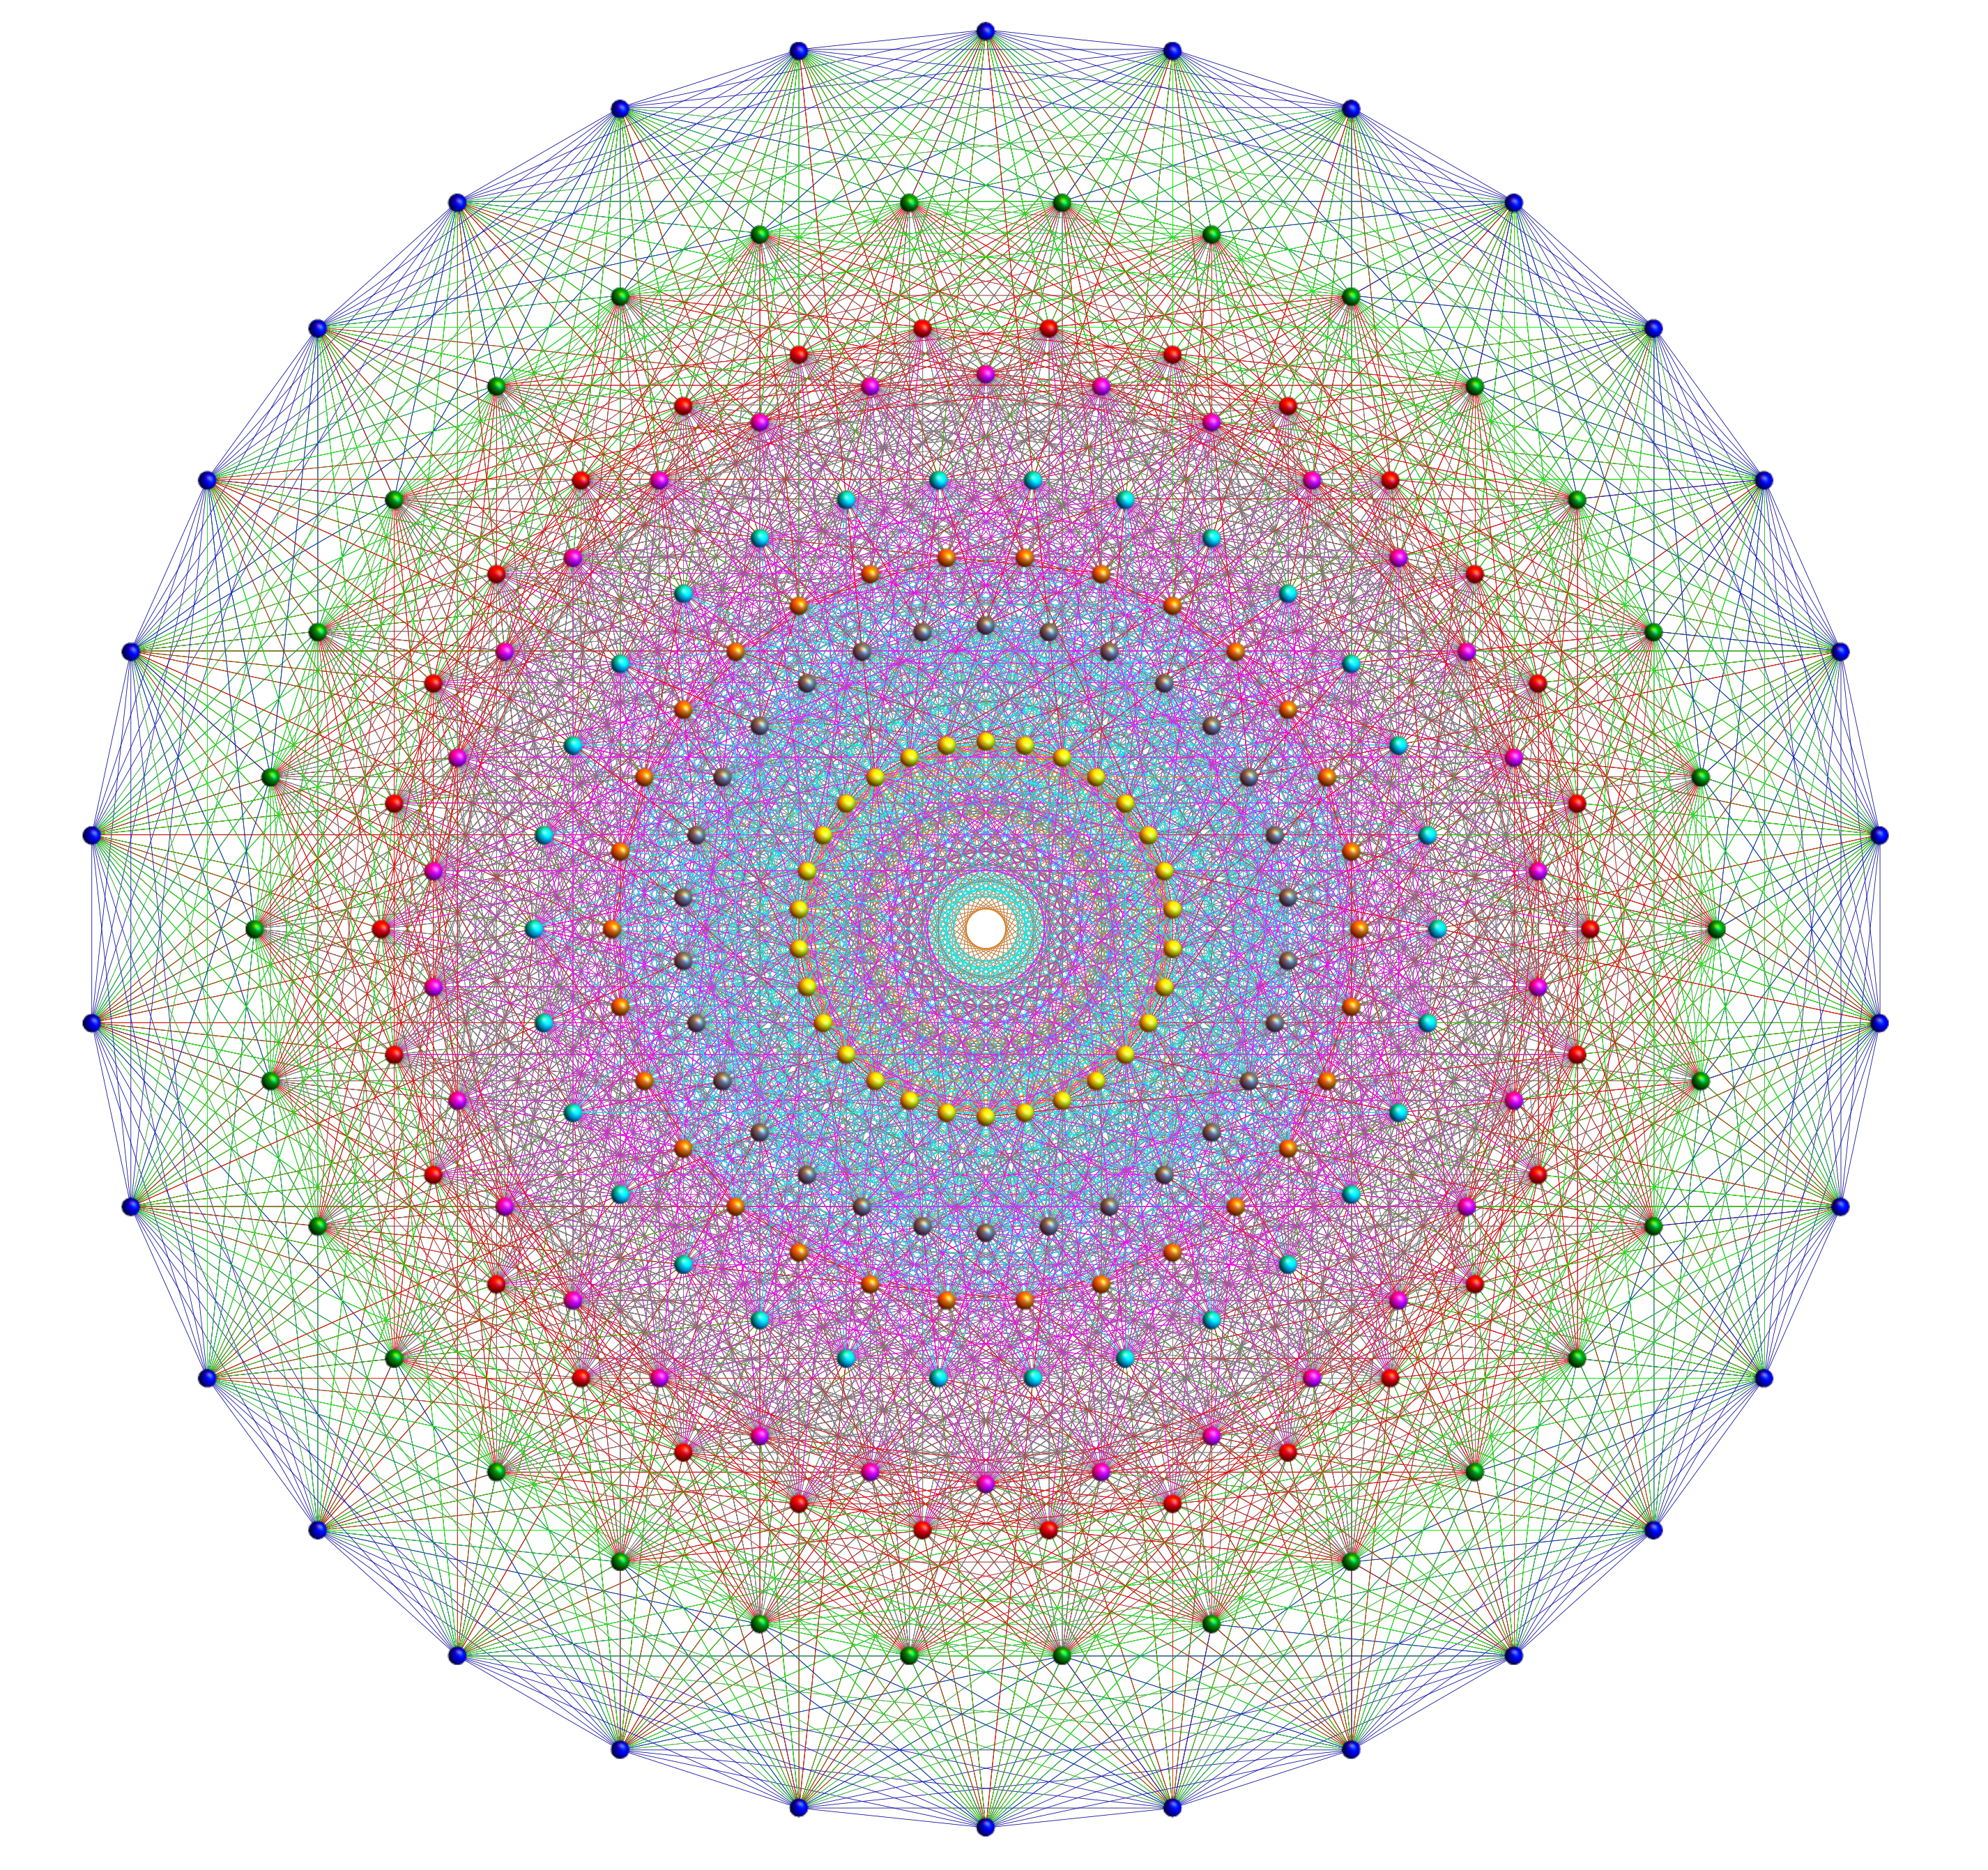
\includegraphics[width=.6\columnwidth]{front.jpg}
\end{figure}

\newpage
\pagestyle{plain}
\tableofcontents 
\newpage
\pagestyle{fancy}
\section{Teoria delle curve}
\subsection{Introduzione}
\begin{definizione}
	[Curva parametrizzata]
	Una \textit{curva paramtrizzata} \`e un'applicazione $\alpha  : I\subset \mathbb{R} \to \mathbb{R}^3$ di classe $C^\infty(I)$, con $I$ intervallo aperto.
	Data $t\in I$, si pu\`o scrivere in componenti come
	\[
	\alpha (t) = (x(t),y(t),z(t))
	\] 
	con $x,y,z:I\to \mathbb{R}$ tutte di classe $C^\infty(I)$.
\end{definizione}
\begin{osservazione}
La necessit\`a di definire la curva su un aperto, o quantomeno di poter estendere l'intervallo di definizione ad un aperto, deriva dal fatto che, in questo modo, si pu\`o effettivamente parlare di derivata piena anche per gli estremi, potendo trovare, infatti, un aperto che contiene interamente i punti di frontiera dell'intervallo di definizione.

Se non si avesse questa possibilit\`a, nel caso di $\alpha :[a,b] \subset \mathbb{R}\to \mathbb{R}^3$, per esempio, non si potrebbe calcolare la derivata tradizionale in $a$, o $b$, perch\'e si potrebbe solamente calcolare il limite destro o sinistro.
\end{osservazione}
\noindent Si nota che, nel caso in cui $I$ non fosse aperto, si estende l'intervallo di definizione ad $A \supset I$ aperto.

Si parla di \textit{traccia} della curva in riferimento all'immagine che genera dell'intero intervallo: $\operatorname{Tr} \alpha  = \alpha (I)$.
La traccia rappresenta l'unione di ciascun punto di $\alpha (t) \in \mathbb{R}^3, \ \forall t \in I$.
Per \textit{velocit\`a} della curva, invece, si intende la grandezza
\begin{equation}
	\alpha '(t) = \lim_{h \to 0} \frac{\alpha (t + h) - \alpha (t)}{h} = \big(x'(t),y'(t),z'(t)\big)
\end{equation}
In realt\`a, questo rappresenta il \textit{vettore velocit\`a}, mentre la velocit\`a vera e propria \`e data dalla sua norma $\left\lVert \alpha' (t) \right\rVert $.
\begin{esempio}
	[Retta parametrizzata]
	Siano $P,Q \in \mathbb{R}^3$, con $P\neq Q$, due punti dello spazio; si definisce, allora, \textit{retta parametrizzata} la curva 
	\[
	\alpha (t) = P + t \overrightarrow{PQ}
	\] 
La sua traccia \`e la retta affine passante per $P$ e $Q$, e ha vettore velocit\`a $\alpha '(t) = \overrightarrow{PQ}$, da cui $\left\lVert \alpha '(t) \right\rVert = \lVert \overrightarrow{PQ} \rVert$, che \`e costante.
\end{esempio}
\begin{esempio}
	[Circonferenza parametrizzata]
Dato $a\in \mathbb{R}$, con $a > 0$, si definisce \textit{circonferenza parametrizzata} come 
\[
\alpha (t) = (a \cos t, a \sin t , 0)
\] 
il cui vettore velocit\`a \`e dato da $\alpha '(t) = (-a\sin t, a \cos t, 0)$, che non risulta costante, mentre la sua velocit\`a $\left\lVert \alpha ' \right\rVert = a >0$ s\`i.
La traccia corrisponde ad una circonferenza nel piano $z=0$, di centro l'origine e raggio $a$.
\end{esempio}
\begin{definizione}
	[Curva regolare]
	Una curva parametrizzata $\alpha : I \subset \mathbb{R} \to \mathbb{R}^3$ \`e detta \textit{regolare} se $\alpha '(t) \neq 0, \ \forall t \in I$.
\end{definizione}
\begin{definizione}
	[Lunghezza d'arco]
	Sia $\alpha  : [a,b] \subset \mathbb{R}\to \mathbb{R}^3$ una curva regolare; si definisce \textit{lunghezza d'arco} la funzione
	\[
	s :
	\begin{array}
		{c c c}
		[a,b] & \longrightarrow &\mathbb{R}\\
		t & \longmapsto &\displaystyle  \int_{a} ^t \left\lVert \alpha '(u) \right\rVert du
	\end{array}
	\] 
	La lunghezza dell'intera curva $\alpha $ \`e data da $L(\alpha ) = s(b)$.
\end{definizione}
\begin{osservazione}
Si nota che per $\alpha : [0,+\infty) \to \mathbb{R}^3$, con $\alpha  (t) = \big(a \cos t, a \sin t, 0\big)$, valendo $\left\lVert \alpha '(t) \right\rVert = a$, si ha:
\[
s(t) = a \int_{0} ^t du = ta \implies s (2\pi) = 2\pi a
\] 
\end{osservazione}
\noindent Sia dato $[a,b] \subset \mathbb{R}$ un intervallo e sia $P \in \mathcal{P} ([a,b])$ una sua partizione, tale che $a = t_0 < t_1 < \ldots<t_{k-1} <t_k = b$; allora la lunghezza di una curva $\alpha  : [a,b] \to \mathbb{R}^3$ approssimata a tale partizione \`e data da:
\begin{equation}
	L(\alpha , P) = \sum_{i=0}^{k-1} \left\lVert \alpha (t_{i+1}) - \alpha (t_i) \right\rVert 
\end{equation}
Si nota, dunque, che la lunghezza effettiva della curva coincide con
\begin{equation}
	\sup_{P \in \mathcal{P}([a,b]) } L(\alpha ,P) = \int_{a} ^b \left\lVert \alpha' (u) \right\rVert du
\end{equation}
Si considera, ancora una curva $\alpha :[a,b] \to \mathbb{R}^3$; visto che $s(t) = \int_{a} ^t \left\lVert \alpha '(u) \right\rVert du$, allora $s'(t) = \left\lVert \alpha '(t) \right\rVert >0$.
Si pu\`o pensare alla lunghezza d'arco come $s : [a,b] \to [0, L(\alpha )]$, che, essendo monotona perch\'e si \`e appena osservato che $s'(t) > 0$, allora ha anche inversa $t : [0,L(\alpha )]\to [a,b]$.
\`E, quindi, possibile definire la funzione 
\begin{equation}
	\beta = \alpha \circ t : [0,L(\alpha )]\to \mathbb{R}^3
\end{equation}
tale che $\operatorname{Tr} (\beta )=\operatorname{Tr} (\alpha ) $ e $\beta (s) = \alpha (t(s))$, per cui
\[
\beta '(s) = \alpha '(t(s)) t'(s) = \frac{\alpha '(t(s))}{s'(t(s))} = \frac{\alpha '(t(s))}{\left\lVert \alpha '(t) \right\rVert }
\] 
per cui $\left\lVert \beta '(s) \right\rVert =1$.
\begin{definizione}
	[Curva p.l.a.]
	Se $\alpha :I\to\mathbb{R}^3$ \`e una curva tale che $\left\lVert \alpha '(t)\right\rVert = 1 , \ \forall t \in I$, allora si dice che \`e \textit{parametrizzata tramite lunghezza d'arco}, o pla.
\end{definizione}
\begin{osservazione}
In base a quanto detto prima, ogni curva regolare \`e \textit{riparametrizzabile tramite lunghezza d'arco}.
\end{osservazione}
\begin{esempio}
	[Elica]
Sia $a > 0$; allora la mappa
\[
\varphi :
\begin{array}
	{c c c}
	\mathbb{R}^2 & \longrightarrow & \mathbb{R}^3\\
	(u,z) &\longmapsto & (a \cos u , a \sin u , z)
\end{array}
\] 
definisce un cilindro di raggio $a$ attorno all'asse $z$.
Preso $b > 0$ e presi i punti $\left\{ (t,bt) \right\} _{t \in \mathbb{R}} $, relativi ad una retta passante per l'origine, aperto, si pu\`o definire la curva 
\[
\alpha (t) = \varphi (t,bt) = (a \cos t , a \sin t , bt)
\] 
che descrive un'\textit{elica destrorsa}, visto che si \`e preso $b>0$\footnote{Fosse stato $b<0$, sarebbe stata un'\textit{elica sinistrorsa}.}, di raggio $a$ e passo $b$.
Si nota che
\[
\alpha '(t) = (-a \sin t, a \cos t , b) \implies \left\lVert \alpha '(t) \right\rVert =\sqrt{a^2 + b^2} > 0, \ \forall t \in \mathbb{R}
\] 
da cui $\alpha $ \`e regolare. 
Restringendola a $[0,+\infty)$, cio\`e considerando $\alpha : [0,+\infty) \to \mathbb{R}^{3} $, si ha:
\[
	s(t) = \int_{0} ^t \sqrt{a^2 + b^2 }  du = t(s) \sqrt{a^2 + b^2} \implies t(s) = \frac{s}{\sqrt{a^2} +b^2}
\] 
quindi:
\[
\begin{split}
		 \beta (s) &= \alpha (t(s)) = a \left(\frac{s}{\sqrt{a^2 + b^2} }\right) \\
	&= \left(a \cos \left(\frac{s}{\sqrt{a^2+b^2} }\right) , a\sin \left(\frac{s}{\sqrt{a^2 + b^2} }\right),\frac{bs}{\sqrt{a^2 + b^2} } \right)
	\end{split} 
\] 
con $\beta $ pla e, conseguentemente, $\beta (\mathbb{R}) = \operatorname{Tr} (\beta ) = \operatorname{Tr} (\alpha ) = \alpha (\mathbb{R})$.
\end{esempio}
\begin{esempio}
	[Ellisse]
	Siano $a,b \in \mathbb{R}\setminus\left\{ 0 \right\} $ e sia 
	\[
	\mathcal{E} _{a,b} = \left\{ (x,y,0) \in \mathbb{R}^3  \ \bigg\lvert \ \frac{x^2}{a^2} + \frac{y^2}{b^2} = 1\right\} \subset \mathbb{R}^3
	\] 
	Si vuole definire una curva $\alpha $ tale che $\operatorname{Tr} \alpha = \mathcal{E} _{a,b} $
	\begin{svolgimento}
		Si nota che $(x /  a , y / b) \in S^1$, cio\`e
	\[
	\frac{x}{a} = \cos t \hspace{1cm}\frac{y}{b} = \sin t
	\] 
	con $S^1$ circonferenza unitaria e $t\in [0,2\pi)$.
	Sia, allora
	\[
\alpha :
	\begin{array}
		{c c c}
		[0,2\pi) &\longrightarrow & \mathbb{R}^3\\
		t & \longmapsto & (a \cos t , b \sin t, 0)
	\end{array}
	\] 
 e si vede che $\operatorname{Tr} \alpha  = \mathcal{E} _{a,b} $.

	\end{svolgimento}
\end{esempio}
\begin{esempio}
Sia 
\[
\mathcal{C}  = \left\{ (x,y,0) \in \mathbb{R}^3  \mid y^2 = x^3 \right\}  \subset \mathbb{R}^3
\] 
Si vuole costruire $\alpha $ tale che $\operatorname{Tr}\alpha  = \mathcal{C} $.
\begin{svolgimento}
	Se si considera la secante $y = tx$, allora $t^2 x^2 = x^3$, ossia $x= t^2$ e $y = t^3$.
	Ne segue che la curva che soddisfa la richiesta \`e $\alpha (t) = (t^2 , t^3,0)$.
\end{svolgimento}
\end{esempio}
\begin{esempio}
Sia 
\[
\mathcal{C}  = \left\{ (x,y,0)  \mid y^2 = x^3 + x^2 \right\} \subset \mathbb{R}^3
\] 
Si vuole costruire una curva $\alpha $ tale che $\operatorname{Tr} \alpha  = \mathcal{C} $.
\begin{svolgimento}
	Si considera, come prima, $y=tx $, da cui $x^3 + x^2(1-t^2) = 0$, da cui si vede che $x = t^2 - 1$ e $y=t^3 -t$, quindi $\alpha (t) = (t^2 - 1, t^3-t,0)$ ({\color{red} da controllare}).
\end{svolgimento}
\end{esempio}
\begin{lemma}\label{lemdif}
	Se $f, g : I \to \mathbb{R}^{3} $ sono due mappe, allora 
	\[
	\left(f(t)\cdot g(t)\right) ' = f'(t) \cdot g(t) + f(t) \cdot g'(t)
	\] 
	\begin{proof}
		Si ha
		\[
		f(t) \cdot g(t) = \sum_{i=1}^{3} f_i(t) g_i(t)
		\] 
	quindi
	\[
	\left(f(t)\cdot g(t)\right) ' = \sum_{i=1}^{3} \left[ f_i'(t)g_i(t) + f_i(t) g_i'(t) \right] 
	\] 
	\end{proof}
\end{lemma}
\begin{definizione}
	[Versore tangente]
	Data una curva riparametrizzabile $\alpha :I \to \mathbb{R}^3$ e la sua riparametrizzazione tramite lunghezza d'arco $\beta (s)$, si definisce il \textit{versore tangente} ad $\alpha $ come $T(s) = \beta '(s)$.
\end{definizione}
\begin{prop}
	Se $\beta :I \to\mathbb{R}^3$ \`e una curva pla, allora $T'(s) \cdot T(s) = 0$.
	\begin{proof}
		Per quanto visto, $\left\lVert T(s) \right\rVert ^2 = T(s) \cdot T(s) = 1$; per il lemma precedente \ref{lemdif}, si ha $2 T'(s) \cdot T(s) = (T(s)\cdot T(s))' = 0 $.
	\end{proof}
\end{prop}
\begin{definizione}
	[Curvatura]
	Data una curva pla $\beta :I\to \mathbb{R}^3$ e il suo versore tangente $T(s)$, allora se ne definisce la \textit{curvatura} come
	\[
	k (s) = \left\lVert T'(s) \right\rVert 
	\] 
\end{definizione}
\subsection{Riferimento di Frenet}


\end{document}

